\documentclass[twoside]{book}

% Packages required by doxygen
\usepackage{fixltx2e}
\usepackage{calc}
\usepackage{doxygen}
\usepackage[export]{adjustbox} % also loads graphicx
\usepackage{graphicx}
\usepackage[utf8]{inputenc}
\usepackage{makeidx}
\usepackage{multicol}
\usepackage{multirow}
\PassOptionsToPackage{warn}{textcomp}
\usepackage{textcomp}
\usepackage[nointegrals]{wasysym}
\usepackage[table]{xcolor}

% Font selection
\usepackage[T1]{fontenc}
\usepackage[scaled=.90]{helvet}
\usepackage{courier}
\usepackage{amssymb}
\usepackage{sectsty}
\renewcommand{\familydefault}{\sfdefault}
\allsectionsfont{%
  \fontseries{bc}\selectfont%
  \color{darkgray}%
}
\renewcommand{\DoxyLabelFont}{%
  \fontseries{bc}\selectfont%
  \color{darkgray}%
}
\newcommand{\+}{\discretionary{\mbox{\scriptsize$\hookleftarrow$}}{}{}}

% Page & text layout
\usepackage{geometry}
\geometry{%
  a4paper,%
  top=2.5cm,%
  bottom=2.5cm,%
  left=2.5cm,%
  right=2.5cm%
}
\tolerance=750
\hfuzz=15pt
\hbadness=750
\setlength{\emergencystretch}{15pt}
\setlength{\parindent}{0cm}
\setlength{\parskip}{3ex plus 2ex minus 2ex}
\makeatletter
\renewcommand{\paragraph}{%
  \@startsection{paragraph}{4}{0ex}{-1.0ex}{1.0ex}{%
    \normalfont\normalsize\bfseries\SS@parafont%
  }%
}
\renewcommand{\subparagraph}{%
  \@startsection{subparagraph}{5}{0ex}{-1.0ex}{1.0ex}{%
    \normalfont\normalsize\bfseries\SS@subparafont%
  }%
}
\makeatother

% Headers & footers
\usepackage{fancyhdr}
\pagestyle{fancyplain}
\fancyhead[LE]{\fancyplain{}{\bfseries\thepage}}
\fancyhead[CE]{\fancyplain{}{}}
\fancyhead[RE]{\fancyplain{}{\bfseries\leftmark}}
\fancyhead[LO]{\fancyplain{}{\bfseries\rightmark}}
\fancyhead[CO]{\fancyplain{}{}}
\fancyhead[RO]{\fancyplain{}{\bfseries\thepage}}
\fancyfoot[LE]{\fancyplain{}{}}
\fancyfoot[CE]{\fancyplain{}{}}
\fancyfoot[RE]{\fancyplain{}{\bfseries\scriptsize Generated by Doxygen }}
\fancyfoot[LO]{\fancyplain{}{\bfseries\scriptsize Generated by Doxygen }}
\fancyfoot[CO]{\fancyplain{}{}}
\fancyfoot[RO]{\fancyplain{}{}}
\renewcommand{\footrulewidth}{0.4pt}
\renewcommand{\chaptermark}[1]{%
  \markboth{#1}{}%
}
\renewcommand{\sectionmark}[1]{%
  \markright{\thesection\ #1}%
}

% Indices & bibliography
\usepackage{natbib}
\usepackage[titles]{tocloft}
\setcounter{tocdepth}{3}
\setcounter{secnumdepth}{5}
\makeindex

% Hyperlinks (required, but should be loaded last)
\usepackage{ifpdf}
\ifpdf
  \usepackage[pdftex,pagebackref=true]{hyperref}
\else
  \usepackage[ps2pdf,pagebackref=true]{hyperref}
\fi
\hypersetup{%
  colorlinks=true,%
  linkcolor=blue,%
  citecolor=blue,%
  unicode%
}

% Custom commands
\newcommand{\clearemptydoublepage}{%
  \newpage{\pagestyle{empty}\cleardoublepage}%
}

\usepackage{caption}
\captionsetup{labelsep=space,justification=centering,font={bf},singlelinecheck=off,skip=4pt,position=top}

%===== C O N T E N T S =====

\begin{document}

% Titlepage & ToC
\hypersetup{pageanchor=false,
             bookmarksnumbered=true,
             pdfencoding=unicode
            }
\pagenumbering{alph}
\begin{titlepage}
\vspace*{7cm}
\begin{center}%
{\Large C\+S2014 Coins (Assignment 3) }\\
\vspace*{1cm}
{\large Generated by Doxygen 1.8.13}\\
\end{center}
\end{titlepage}
\clearemptydoublepage
\pagenumbering{roman}
\tableofcontents
\clearemptydoublepage
\pagenumbering{arabic}
\hypersetup{pageanchor=true}

%--- Begin generated contents ---
\chapter{C\+S2014 2017 Assignment3 -\/ Moar crypto, of the play-\/coin variety}
\label{md_README}
\Hypertarget{md_README}
our basic cs2094 coin type

Your assignment is to write code that creates bitcoin-\/like values that meet the spec below and that are verified by the code you\textquotesingle{}re given here. What we\textquotesingle{}ll be doing is actually more like a \href{https://www.bitcoinmining.com/what-is-hashcash/}{\tt hashcash proof-\/of-\/work} rather than anything to do with the bitcoin blockchain.

We\textquotesingle{}ll re-\/use the \href{https://tls.mbed.org/kb}{\tt mbed T\+LS} package for the verifier code. You pretty much have to do the same for the coin making code so that the automated assignment marking system works. There are some hints below to which you ought pay attention.

\subsection*{To setup a working environment...}

See \href{../assignment2/README.html}{\tt assignment2}.

If you clone the course repo and this file is in {\ttfamily \$\+R\+E\+PO/assignments/assignment3} then that directory contains a Makefile you can use. That Makefile assumes that you already built mbed T\+LS for assignment 2 and that the mbed T\+LS header files and library are below {\ttfamily \$\+R\+E\+PO/assignments/assignment2} -\/ if you used some other directory structure you\textquotesingle{}ll need to figure out what to change.

\subsection*{\char`\"{}\+C\+S2014 C\+O\+I\+N\char`\"{} Specification}

\subsubsection*{Overview}

The basic idea is similar to, but a lot simpler than, the bitcoin idea of mining \href{https://en.bitcoin.it/wiki/Difficulty}{\tt \char`\"{}difficulty\char`\"{}}. We require that each \char`\"{}\+C\+S2014 coin\char`\"{} be unique and include the inputs to a S\+H\+A256 hash whose output value has a selected number of the low order (rightmost) bits with zero values. Since the output of a hash function like S\+H\+A256 is essentially random, one has to try many times before one sees such an output, and the longer the run of zeros required, the more attempts one needs.

To generate such outputs we include a \href{https://en.wikipedia.org/wiki/Cryptographic_nonce}{\tt cryptographic nonce} in the hash input value. We can vary the nonce value until we find a hash output with the required number of bits zero-\/valued. (Efficiency in coin mining is clearly important, so please do try to make your code for this part as speedy as you can! Some marks may be available for that -\/ ping me if you think you\textquotesingle{}ve written some notably good code.)

In addition (just for the coding fun\+:-\/) we require each coin to be digitally signed using the Elliptic Curve Digital Signature Algorithm (E\+C\+D\+SA) with the p256 N\+I\+ST curve. (That\textquotesingle{}s the default when you generate an Elliptic Curve key pair, so you won\textquotesingle{}t need to understand any details of E\+C\+D\+SA\+:-\/) Our coins therefore also include the public key needed to verify the coin signature in the signed data.

There are also some housekeeping fields to help with encoding and decoding and for (pretend\+:-\/) futureproofing.

C\+S2014 coins are binary values. We don\textquotesingle{}t use J\+S\+ON, X\+ML or any other generic data representation scheme.

\subsubsection*{Example}

Here\textquotesingle{}s a hexdump of an example coin with 20 bits of difficulty\+: \begin{DoxyVerb}    00,00,00,00,00,00,00,14,00,00,00,9e,30,81,9b,30
    10,06,07,2a,86,48,ce,3d,02,01,06,05,2b,81,04,00
    23,03,81,86,00,04,01,c8,46,55,6b,4e,26,bb,6e,22
    d8,7a,f8,2e,1b,15,0b,18,af,98,33,59,00,66,d9,0c
    08,63,75,4a,ea,50,5e,54,7e,72,8e,3d,57,cb,89,15
    0f,bc,10,0b,5a,1b,3a,84,08,9f,73,0a,e7,38,c7,03
    e4,2e,1a,19,45,08,25,f8,01,bd,89,0f,3a,e1,18,3a
    87,51,74,71,94,a2,4c,8a,1e,3a,7c,52,f3,03,6e,91
    fe,97,42,4f,3e,22,b7,c5,72,8c,f8,da,dd,53,ee,42
    ca,af,8d,78,38,70,10,63,e9,8c,51,a5,02,f2,89,f8
    a0,4d,68,7a,a5,96,d4,67,70,12,00,00,00,20,1e,a9
    86,c4,2b,ff,9f,99,00,2d,be,2e,91,c4,5a,ac,b7,49
    e4,7e,1a,7f,65,ae,29,bf,3f,c7,d0,c5,ce,39,00,00
    00,20,2c,55,ee,bd,2c,f0,ad,c8,77,56,cf,b6,15,e8
    5e,2b,18,ce,3e,5c,fc,56,d2,4f,9a,8b,f5,71,a5,10 <- 20 zero bits start with that last nibble 
    00,00,00,00,00,8a,30,81,87,02,41,3b,cb,b3,10,9a
    87,03,89,ec,61,aa,e4,9c,83,1a,7e,27,64,5b,6d,74
    fc,6c,a7,f2,f9,2c,1c,11,c6,56,76,b2,77,aa,92,c8
    cf,de,e8,9d,0f,0f,e3,c0,7a,5b,8f,04,e0,a2,7d,af
    70,27,57,fb,4b,ba,3d,48,c2,fa,e5,ee,02,42,01,86
    ff,a4,93,1e,ba,18,f5,14,65,06,25,86,10,9c,d7,3e
    53,30,c9,39,a3,90,13,b2,7f,a1,ba,10,af,5b,53,c8
    b1,ae,6a,19,ed,2a,a3,3a,ec,8b,01,7c,50,9a,15,8b
    7a,77,7b,28,b4,70,71,1f,77,40,c2,6b,22,0e,6e,fb
\end{DoxyVerb}


\subsubsection*{Protocol data units (P\+D\+Us)}

Our coin syntax is pretty simple, with all but one field being fixed width (for now), and hence doesn\textquotesingle{}t need us to use any data definition language such as \href{https://en.wikipedia.org/wiki/Abstract_Syntax_Notation_One}{\tt A\+S\+N.\+1}, \href{https://en.wikipedia.org/wiki/XML_schema}{\tt X\+ML schema} etc.

The fields in a C\+S2014 coin are\+:

\tabulinesep=1mm
\begin{longtabu} spread 0pt [c]{*{4}{|X[-1]}|}
\hline
\rowcolor{\tableheadbgcolor}\textbf{ Offset}&\textbf{ Name}&\textbf{ Length}&\textbf{ Description }\\\cline{1-4}
\endfirsthead
\hline
\endfoot
\hline
\rowcolor{\tableheadbgcolor}\textbf{ Offset}&\textbf{ Name}&\textbf{ Length}&\textbf{ Description }\\\cline{1-4}
\endhead
0&Ciphersuite&4&Specifies all cryptographic algorithms -\/ value for now fixed at zero \\\cline{1-4}
4&Bits&4&Specifies difficulty \\\cline{1-4}
8&Public Key length&4&Specifies length of public key \\\cline{1-4}
12&Public Key&158&Public key value (fixed for p256 curve) \\\cline{1-4}
170&Nonce len&4&length of nonce \\\cline{1-4}
174&Nonce&32&nonce used to generate PoW hash \\\cline{1-4}
206&PoW Hash len&4&length of proof-\/of-\/work hash \\\cline{1-4}
210&PoW Hash&32&proof-\/of-\/work hash \\\cline{1-4}
242&Signature len&4&length of coin self-\/signature \\\cline{1-4}
246&Signature&Variable ($\sim$138 octets)&coin self-\/signature \\\cline{1-4}
\end{longtabu}


The ciphersuite value of zero means\+: \char`\"{}use S\+H\+A256 for the proof-\/of-\/work and use
\+E\+C\+D\+S\+A with N\+I\+S\+T p256 for the public key and signature.\char`\"{} The ciphersuite concept is used in T\+LS and various other cryptographic protocols.

All length fields and the bits field are in \href{https://en.wikipedia.org/wiki/Network_byte_order}{\tt network byte order}.

As a side-\/note\+: the public key and signature fields do actually internally use A\+S\+N.\+1 specified encoding of those values encoded with the Distiguished Encoding Rules (\href{https://en.wikipedia.org/wiki/Distinguished_Encoding_Rules}{\tt D\+ER}). That\textquotesingle{}s done so that those are the same values used in \href{https://tools.ietf.org/html/rfc5280}{\tt X.\+509 public key certificates}, as used for Transport Layer Security (\href{https://tools.ietf.org/html/rfc5246}{\tt T\+LS}), e.\+g. when using \href{https://tools.ietf.org/html/rfc2818}{\tt H\+T\+T\+PS}. While we don\textquotesingle{}t notice it here, that actually makes those values more complex and bigger for no ostensibly good reason, if one didn\textquotesingle{}t consider the savings in code re-\/use. Cases like that are common, and are one reason why it can take a very loooong time to migrate away from use of some pretty old format/\+A\+PI to any shiny new format/\+A\+PI. (See issues with \href{https://cryptosense.com/why-pkcs1v1-5-encryption-should-be-put-out-of-our-misery/}{\tt P\+K\+CS\#1v1.\+5}.)

\subsubsection*{Cryptographic inputs/outputs}


\begin{DoxyItemize}
\item Bytes 0..205 inclusive are input to the Proof-\/of-\/\+Work (PoW) hash (which uses S\+H\+A256).
\item Bytes 206..241 inclusive are the PoW length and hash value
\item Bytes 0..241 inclusive are input to the signature
\item Bytes 242..end are the signature length and value
\end{DoxyItemize}

\subsubsection*{Example (again)}

Breaking the above sample down into these fields we get... \begin{DoxyVerb}    Ciphersuite (0)
    00,00,00,00,
    Difficulty in terms of bits (20)
                00,00,00,14,
    Length of public key (4)
                            00,00,00,9e,
    Public key value (158, DER encoded)
                                        30,81,9b,30
    10,06,07,2a,86,48,ce,3d,02,01,06,05,2b,81,04,00
    23,03,81,86,00,04,01,c8,46,55,6b,4e,26,bb,6e,22
    d8,7a,f8,2e,1b,15,0b,18,af,98,33,59,00,66,d9,0c
    08,63,75,4a,ea,50,5e,54,7e,72,8e,3d,57,cb,89,15
    0f,bc,10,0b,5a,1b,3a,84,08,9f,73,0a,e7,38,c7,03
    e4,2e,1a,19,45,08,25,f8,01,bd,89,0f,3a,e1,18,3a
    87,51,74,71,94,a2,4c,8a,1e,3a,7c,52,f3,03,6e,91
    fe,97,42,4f,3e,22,b7,c5,72,8c,f8,da,dd,53,ee,42
    ca,af,8d,78,38,70,10,63,e9,8c,51,a5,02,f2,89,f8
    a0,4d,68,7a,a5,96,d4,67,70,12,
    Length of Nonce (4)
                                  00,00,00,20,
    Nonce value (32)
                                              1e,a9
    86,c4,2b,ff,9f,99,00,2d,be,2e,91,c4,5a,ac,b7,49
    e4,7e,1a,7f,65,ae,29,bf,3f,c7,d0,c5,ce,39,
    Length of Proof-of-Work hash (4)
                                              00,00
    00,20,
    Proof-of-Work hash (32)
          2c,55,ee,bd,2c,f0,ad,c8,77,56,cf,b6,15,e8
    5e,2b,18,ce,3e,5c,fc,56,d2,4f,9a,8b,f5,71,a5,10
    00,00,
    Length of Signature (4)
          00,00,00,8a,
    Signature (138, DER encoded)
                      30,81,87,02,41,3b,cb,b3,10,9a
    87,03,89,ec,61,aa,e4,9c,83,1a,7e,27,64,5b,6d,74
    fc,6c,a7,f2,f9,2c,1c,11,c6,56,76,b2,77,aa,92,c8
    cf,de,e8,9d,0f,0f,e3,c0,7a,5b,8f,04,e0,a2,7d,af
    70,27,57,fb,4b,ba,3d,48,c2,fa,e5,ee,02,42,01,86
    ff,a4,93,1e,ba,18,f5,14,65,06,25,86,10,9c,d7,3e
    53,30,c9,39,a3,90,13,b2,7f,a1,ba,10,af,5b,53,c8
    b1,ae,6a,19,ed,2a,a3,3a,ec,8b,01,7c,50,9a,15,8b
    7a,77,7b,28,b4,70,71,1f,77,40,c2,6b,22,0e,6e,fb
\end{DoxyVerb}


\subsubsection*{Some implementation requirements}

The specification above is basically a functional requrements specification that says what your code must do. In addition, and as is common, we also have some implementation requirements that \href{https://tools.ietf.org/html/rfc2119}{\tt M\+U\+ST} also be met\+:


\begin{DoxyItemize}
\item Your implementation M\+U\+ST honour the existing A\+PI defined in \href{./cs2014coin.h}{\tt cs2014coin.\+h}
\item Your implementation M\+U\+ST honour the existing command line arguments defined in \href{./cs2014coin-main.c}{\tt cs2014coin-\/main.\+c}
\item Coins produced by your implementation M\+U\+ST be verifiable using the verification implementation you\textquotesingle{}ve been given. (That is, you cannot just change the verifier to win the game\+:-\/)
\item Your implementation of a coin miner S\+H\+O\+U\+LD honour the C\+S2014\+C\+O\+I\+N\+\_\+\+M\+A\+X\+I\+T\+E\+RS value defined in the A\+PI -\/ that means your code ought exit with an error if it doesn\textquotesingle{}t find a coin after that number of iterations of nonce values.
\item You S\+H\+O\+U\+LD implement your coin miner in one .c file, it\textquotesingle{}d make sense to keep using the \href{./cs2014coin-make.c}{\tt cs2014coin-\/make.\+c} file and just add your code to that.
\end{DoxyItemize}

\subsubsection*{Some hints...}

Here\textquotesingle{}s a few hints to help you with your mining code\+:


\begin{DoxyItemize}
\item There are examples in {\ttfamily \$\+B\+U\+I\+LD/mbedtls-\/2.6.\+0/programs/pkey/} that should help you figure out how to use the mbed T\+LS A\+P\+Is. (But you\textquotesingle{}ve a bunch of stuff to figure out too!) Don\textquotesingle{}t only stare at that code -\/ build, run and test it too.
\item mbed T\+LS functions you will likely want to use will include\+:
\begin{DoxyItemize}
\item {\ttfamily mbedtls\+\_\+ctr\+\_\+drbg\+\_\+seed}
\item {\ttfamily mbedtls\+\_\+ecp\+\_\+gen\+\_\+key}
\item {\ttfamily mbedtls\+\_\+md\+\_\+starts}
\item {\ttfamily mbedtls\+\_\+md\+\_\+update}
\item {\ttfamily mbedtls\+\_\+md\+\_\+finish}
\item {\ttfamily mbedtls\+\_\+pk\+\_\+sign}
\end{DoxyItemize}
\item There are also various {\ttfamily mbedtls\+\_\+$\ast$\+\_\+init} and {\ttfamily mbedtls\+\_\+$\ast$\+\_\+setup} functions related to the above that you\textquotesingle{}ll need to call to get those to work properly.
\item Using network byte order means calls to {\ttfamily htonl} and {\ttfamily ntohl} are needed, in case the miner\textquotesingle{}s and verifier\textquotesingle{}s machines have different endianness.
\item The {\ttfamily hexdump} (aka {\ttfamily hd}) tool will help you see what you\textquotesingle{}re putting in files, e.\+g. to check if your lengths are or are not in network byte order.
\item Writing your code to test with a small value for \char`\"{}bits\char`\"{} (say 5) will help
\item Until your code seems to be working, limiting the iterations to a small number (say 2) will help you debug your stuff
\item You\textquotesingle{}ll likely need to debug with {\ttfamily gdb} for this one. We\textquotesingle{}ll chat about that in class.
\item My working implementation of {\ttfamily \hyperlink{cs2014coin-make_8c}{cs2014coin-\/make.\+c}} has 250 lines in the file, including comments and debugging code. Yours shouldn\textquotesingle{}t be too much different to that.
\item Understanding the verification code will help you write the mining code, so don\textquotesingle{}t ignore that. You can run it and debug it using the sample coin.
\item Once you have a working coin miner, then you should be able to use the \href{./check-timing.sh}{\tt check-\/timing.\+sh} shell script to see if your performance, (in terms of iterations of attempted proof-\/of-\/work), is roughly similar to openssl\textquotesingle{}s sha256 (in hashes per second) on your development box. They should be close -\/ less than an order of magnitude apart.
\end{DoxyItemize}

\subsection*{A typedef for our coins...}

The \href{./cs2014coin.h}{\tt cs2014coin.\+h} header file defines the A\+PI you have to use, and includes the {\ttfamily typedef struct} below. You can, but don\textquotesingle{}t have to use that in your code. (There are no copies of, or pointers to, instances of that structure passed in the A\+PI, so you don\textquotesingle{}t have to use it.)

But we\textquotesingle{}ll look at it now anyway... \begin{DoxyVerb}    /*!
     *       * 
     * This structure describes a cs2014 coin.
     * Fields are flattened as usual, lengths use network byte order.
     * The hash is over the fields that preceed it in the struct.
     * The rightmost 'bits' bits of the hash value must be zero.
     * The signature is over the fields that proceed it in the struct.
     * All length fields, except 'bits' are in octets
     *
     */
    typedef struct cs2014coin_t_defn {
        int ciphersuite; /// specifies all algorithms 
        int bits; /// specifies the zero-bit run length needed in the hashval
        int keylen; /// length of the public key
        unsigned char *keyval; /// public key value
        int noncelen; /// length of nonce
        unsigned char *nonceval;
        int hashlen; /// length of hashval
        unsigned char *hashval; /// hash value with 'bits' of the LSBs having a value of zero 
        int siglen; /// signature length
        unsigned char *sigval; /// signature value
    } cs2014coin_t;
\end{DoxyVerb}


If I wanted to use that in some code, then I\textquotesingle{}d declare a variable {\ttfamily mycoin} like this\+: \begin{DoxyVerb}    cs2014coin_t mycoin;
\end{DoxyVerb}


And I can access (read/set) the field values like this\+: \begin{DoxyVerb}    mycoin.ciphersuite==CS2014COIN_CS_0;
\end{DoxyVerb}


When I declare such a variable on the stack it\textquotesingle{}ll consume a pile of memory ( 6 ints and 4 pointers, so maybe $\sim$48 bytes total or more if the compiler aligns things specially). But your code may be a good bit tidier if you use such a variable rather than have a load of separate variables (which won\textquotesingle{}t really be much more memory efficient in many cases). And tidier code is easier to maintain etc. which is a good thing (tm).

If I wanted to pass a value like mycoin (say after it\textquotesingle{}s been fully populated) to some function, {\ttfamily print\+\_\+coin()} then I might declare that function like this\+: \begin{DoxyVerb}    void print_coin (cs2014coin_t coin);
\end{DoxyVerb}


To call that with mycoin as an input I just pass the variable to the function follows\+: \begin{DoxyVerb}    print_coin(mycoin);
\end{DoxyVerb}


That\textquotesingle{}s a little inefficient as the full structure is passed on the stack. So we much more commonly pass a pointer to the structure and hence would have a function like this instead\+: \begin{DoxyVerb}    void print_coin (cs2014coin_t *coin);
\end{DoxyVerb}


Now there\textquotesingle{}s only one pointer passed on the stack which is better, for large structs. To call that with mycoin as an input I need to pass the address of mycoin and not the value of mycoin, which I do using the \& character as follows\+: \begin{DoxyVerb}    print_coin(&mycoin);
\end{DoxyVerb}


Inside that function, to access (read/set) the values of the fields we might have code like\+:

\begin{DoxyVerb}    if (coin->ciphersuite==CS2014COIN_CS_0) {
        printf("Default Cipersuite\n");
    }
\end{DoxyVerb}


There\textquotesingle{}s also an {\itshape important} difference in passing things or pointers to things to functions. Since C passes everything {\itshape by value}, you have to pass a pointer to that thing if the function you\textquotesingle{}re calling needs to modify the value of an input. (To make a parameter an in/out parameter in e.\+g. doxygen terms.)

I like \href{https://denniskubes.com/2012/08/20/is-c-pass-by-value-or-reference/}{\tt this} description of how C does pass by value.

But again, you might or might not want to use this particular struct in doing assignment 3, I mainly included it to have this discussion of {\itshape pass by value} and {\itshape pass by reference}.

\subsection*{What\textquotesingle{}s here?}

The files in this assignment directory you should see now are\+:


\begin{DoxyItemize}
\item \href{cs2014.coin}{\tt cs2014.\+coin} -\/ a sample coin
\item \href{cs2014coin-main.c}{\tt cs2014coin-\/main.\+c} -\/ the main line code
\item \href{cs201coin.h}{\tt cs2014coin.\+h} -\/ the A\+PI definition
\item \href{cs201coin.h}{\tt cs2014coin-\/int.\+h} -\/ macros and function prototypes used internally by the A\+PI implementation
\item \href{cs2014coin-check.c}{\tt cs2014coin-\/util.\+c} -\/ some A\+PI utilities
\item \href{cs2014coin-check.c}{\tt cs2014coin-\/check.\+c} -\/ the A\+PI implementation code for coin checking
\item \href{cs2014coin-make.c}{\tt cs2014coin-\/make.\+c} -\/ a stub of the A\+PI implementation code for making coins -\/ you\textquotesingle{}ll write the code for this
\item \href{./check-timing.sh}{\tt check-\/timing.\+sh} -\/ a script to see how fast/slow we are vs. openssl
\item \mbox{[}Makefile\mbox{]}(Makefile) -\/ the Makefile to builld the above and link in the mbed T\+LS library
\item \href{./refman.pdf}{\tt refman.\+pdf} -\/ the Doxygen P\+DF documentation for this project
\item \href{../assignment2/mbedtls-2.6.0/}{\tt ../assignment2/mbedtls-\/2.6.\+0} -\/ the directory with the mbed T\+LS stuff
\item \href{https://tls.mbed.org/download/start/mbedtls-2.6.0-apache.tgz}{\tt ../assignment2/mbedtls-\/2.6.\+0-\/apache.\+tgz}-\/ the tarball you downloaded
\item \href{README.html}{\tt R\+E\+A\+D\+M\+E.\+html} -\/ this H\+T\+ML file
\item \hyperlink{md_README}{R\+E\+A\+D\+ME.md} -\/ the markdown source for this H\+T\+ML file
\end{DoxyItemize}

\subsection*{Noteworthy}

There are a number of notewothy things in the code given to you for this assignment\+:


\begin{DoxyItemize}
\item We\textquotesingle{}ve seen our first use of an \href{https://tools.ietf.org/html/rfc2119}{\tt R\+F\+C2119} M\+U\+ST
\item We\textquotesingle{}ve used {\ttfamily extern} in the internal A\+PI stuff for error strings.
\item We use {\ttfamily getopt()} -\/ for details see {\ttfamily man 3 getopt} Do also look at this \href{https://www.gnu.org/software/libc/manual/html_node/Example-of-Getopt.html}{\tt example}
\item The verification \href{./cs2014coin-check.c}{\tt code} attempts to be \href{https://cryptocoding.net/index.php/Coding_rules}{\tt constant time}. That code is nearly, but not quite, done -\/ anyone interested in improving that is welcome to try and I\textquotesingle{}ll be interested in what you find. (I might do a bit more on that myself as I need to learn how to do sometime\+:-\/)
\item {\ttfamily \hyperlink{cs2014coin-int_8h_afd151090a1b9f8e9a800daa05be4bbf6}{dumpbuf()}} etc is handy and fairly typical
\item Things like {\ttfamily \hyperlink{cs2014coin-int_8h}{cs2014coin-\/int.\+h}} and {\ttfamily \hyperlink{cs2014coin-util_8c}{cs2014coin-\/util.\+c}} are typical too.
\item Error string handling like this is sorta-\/but-\/not-\/that common
\item The doxygen docs for this could be interesting to look at, see if you can make them?
\item I\textquotesingle{}d have preferred to use \href{https://en.wikipedia.org/wiki/EdDSA}{\tt Ed\+D\+SA}, and in particular \href{https://tools.ietf.org/html/rfc8032}{\tt Ed25519}, for this, or at least \href{https://tools.ietf.org/html/rfc6979}{\tt deterministic signatures}, but that\textquotesingle{}d have made this too hard an assignment. The reason is that E\+C\+D\+SA signature generation requires a random number, and if that\textquotesingle{}s badly chosen, then the private signing key can leak (invalidating the entire point of signing). Such details are often not easily visible to you as a programmer, but can be critically important for the overall system produced. (The point here is about security, but similar issues arise for any emergent property of the system, such as performance or usability.)
\end{DoxyItemize}

\subsection*{Deadline}

The deadline for submission of this assignment is 2017-\/10-\/30

\subsection*{Submission}

For this assignment you should only submit your single file of source code, which can be called {\ttfamily \hyperlink{cs2014coin-make_8c}{cs2014coin-\/make.\+c}}

To submit your assignment use \href{https://cs2014.scss.tcd.ie/}{\tt https\+://cs2014.\+scss.\+tcd.\+ie/} as usual. 
\chapter{Class Index}
\section{Class List}
Here are the classes, structs, unions and interfaces with brief descriptions\+:\begin{DoxyCompactList}
\item\contentsline{section}{\hyperlink{structcs2014coin__t__defn}{cs2014coin\+\_\+t\+\_\+defn} \\*Our basic cs2094 coin type }{\pageref{structcs2014coin__t__defn}}{}
\end{DoxyCompactList}

\chapter{File Index}
\section{File List}
Here is a list of all documented files with brief descriptions\+:\begin{DoxyCompactList}
\item\contentsline{section}{\hyperlink{cs2014coin-check_8c}{cs2014coin-\/check.\+c} \\*This is the implemetation of the cs2014 coin checker }{\pageref{cs2014coin-check_8c}}{}
\item\contentsline{section}{\hyperlink{cs2014coin-int_8h}{cs2014coin-\/int.\+h} \\*Definitions/macros used internally }{\pageref{cs2014coin-int_8h}}{}
\item\contentsline{section}{\hyperlink{cs2014coin-main_8c}{cs2014coin-\/main.\+c} \\*This is the main function for cs2014 coin handling }{\pageref{cs2014coin-main_8c}}{}
\item\contentsline{section}{\hyperlink{cs2014coin-make_8c}{cs2014coin-\/make.\+c} \\*This is the implementation of the cs2014 coin maker }{\pageref{cs2014coin-make_8c}}{}
\item\contentsline{section}{\hyperlink{cs2014coin-util_8c}{cs2014coin-\/util.\+c} \\*This is the implementation of utilities for cs2014 coins }{\pageref{cs2014coin-util_8c}}{}
\item\contentsline{section}{\hyperlink{cs2014coin_8h}{cs2014coin.\+h} \\*This is the external i/f for the cs2014 coin example }{\pageref{cs2014coin_8h}}{}
\end{DoxyCompactList}

\chapter{Class Documentation}
\hypertarget{structcs2014coin__t__defn}{}\section{cs2014coin\+\_\+t\+\_\+defn Struct Reference}
\label{structcs2014coin__t__defn}\index{cs2014coin\+\_\+t\+\_\+defn@{cs2014coin\+\_\+t\+\_\+defn}}


our basic cs2094 coin type  




{\ttfamily \#include $<$cs2014coin.\+h$>$}

\subsection*{Public Attributes}
\begin{DoxyCompactItemize}
\item 
\mbox{\Hypertarget{structcs2014coin__t__defn_a0a3f3ed501a085bbc195882ce031a0af}\label{structcs2014coin__t__defn_a0a3f3ed501a085bbc195882ce031a0af}} 
int \hyperlink{structcs2014coin__t__defn_a0a3f3ed501a085bbc195882ce031a0af}{ciphersuite}
\begin{DoxyCompactList}\small\item\em specifies all algorithms \end{DoxyCompactList}\item 
\mbox{\Hypertarget{structcs2014coin__t__defn_abb73ecea0a002525acb824f17978725c}\label{structcs2014coin__t__defn_abb73ecea0a002525acb824f17978725c}} 
int \hyperlink{structcs2014coin__t__defn_abb73ecea0a002525acb824f17978725c}{bits}
\begin{DoxyCompactList}\small\item\em specifies the zero-\/bit run length needed in the hashval \end{DoxyCompactList}\item 
\mbox{\Hypertarget{structcs2014coin__t__defn_a451ffb33473c5af67e64fde5f991bdfa}\label{structcs2014coin__t__defn_a451ffb33473c5af67e64fde5f991bdfa}} 
int \hyperlink{structcs2014coin__t__defn_a451ffb33473c5af67e64fde5f991bdfa}{keylen}
\begin{DoxyCompactList}\small\item\em length of the public key \end{DoxyCompactList}\item 
\mbox{\Hypertarget{structcs2014coin__t__defn_af77bb1c315c160ac696ad26e7d4c74b4}\label{structcs2014coin__t__defn_af77bb1c315c160ac696ad26e7d4c74b4}} 
unsigned char $\ast$ \hyperlink{structcs2014coin__t__defn_af77bb1c315c160ac696ad26e7d4c74b4}{keyval}
\begin{DoxyCompactList}\small\item\em public key value \end{DoxyCompactList}\item 
\mbox{\Hypertarget{structcs2014coin__t__defn_a5d529f678ef0f035ca32dff4665da144}\label{structcs2014coin__t__defn_a5d529f678ef0f035ca32dff4665da144}} 
int \hyperlink{structcs2014coin__t__defn_a5d529f678ef0f035ca32dff4665da144}{noncelen}
\begin{DoxyCompactList}\small\item\em length of nonce \end{DoxyCompactList}\item 
\mbox{\Hypertarget{structcs2014coin__t__defn_add7ffdae6b0118288b17915fdbf683f0}\label{structcs2014coin__t__defn_add7ffdae6b0118288b17915fdbf683f0}} 
unsigned char $\ast$ {\bfseries nonceval}
\item 
\mbox{\Hypertarget{structcs2014coin__t__defn_a211e649505f46b21df016560bc3436db}\label{structcs2014coin__t__defn_a211e649505f46b21df016560bc3436db}} 
int \hyperlink{structcs2014coin__t__defn_a211e649505f46b21df016560bc3436db}{hashlen}
\begin{DoxyCompactList}\small\item\em length of hashval \end{DoxyCompactList}\item 
\mbox{\Hypertarget{structcs2014coin__t__defn_a09793a60685db1da70a2286fc8b830d0}\label{structcs2014coin__t__defn_a09793a60685db1da70a2286fc8b830d0}} 
unsigned char $\ast$ \hyperlink{structcs2014coin__t__defn_a09793a60685db1da70a2286fc8b830d0}{hashval}
\begin{DoxyCompactList}\small\item\em hash value with \textquotesingle{}bits\textquotesingle{} of the L\+S\+Bs having a value of zero \end{DoxyCompactList}\item 
\mbox{\Hypertarget{structcs2014coin__t__defn_a05de8a4c54de475945bc4611b8cd743b}\label{structcs2014coin__t__defn_a05de8a4c54de475945bc4611b8cd743b}} 
int \hyperlink{structcs2014coin__t__defn_a05de8a4c54de475945bc4611b8cd743b}{siglen}
\begin{DoxyCompactList}\small\item\em signature length \end{DoxyCompactList}\item 
\mbox{\Hypertarget{structcs2014coin__t__defn_a7f4784554e4643461c6d78775703318f}\label{structcs2014coin__t__defn_a7f4784554e4643461c6d78775703318f}} 
unsigned char $\ast$ \hyperlink{structcs2014coin__t__defn_a7f4784554e4643461c6d78775703318f}{sigval}
\begin{DoxyCompactList}\small\item\em signature value \end{DoxyCompactList}\end{DoxyCompactItemize}


\subsection{Detailed Description}
our basic cs2094 coin type 

This structure describes a cs2014 coin. Fields are flattened as usual, lengths use network byte order. The hash is over the fields that preceed it in the struct. The rightmost \textquotesingle{}bits\textquotesingle{} bits of the hash value must be zero. The signature is over the fields that proceed it in the struct. All length fields, except \textquotesingle{}bits\textquotesingle{} are in octets 

The documentation for this struct was generated from the following file\+:\begin{DoxyCompactItemize}
\item 
\hyperlink{cs2014coin_8h}{cs2014coin.\+h}\end{DoxyCompactItemize}

\chapter{File Documentation}
\hypertarget{cs2014coin-check_8c}{}\section{cs2014coin-\/check.c File Reference}
\label{cs2014coin-check_8c}\index{cs2014coin-\/check.\+c@{cs2014coin-\/check.\+c}}


This is the implemetation of the cs2014 coin checker.  


{\ttfamily \#include $<$stdio.\+h$>$}\newline
{\ttfamily \#include $<$string.\+h$>$}\newline
{\ttfamily \#include $<$arpa/inet.\+h$>$}\newline
{\ttfamily \#include $<$mbedtls/error.\+h$>$}\newline
{\ttfamily \#include $<$mbedtls/md.\+h$>$}\newline
{\ttfamily \#include $<$mbedtls/pk.\+h$>$}\newline
{\ttfamily \#include \char`\"{}cs2014coin.\+h\char`\"{}}\newline
{\ttfamily \#include \char`\"{}cs2014coin-\/int.\+h\char`\"{}}\newline
Include dependency graph for cs2014coin-\/check.c\+:\nopagebreak
\begin{figure}[H]
\begin{center}
\leavevmode
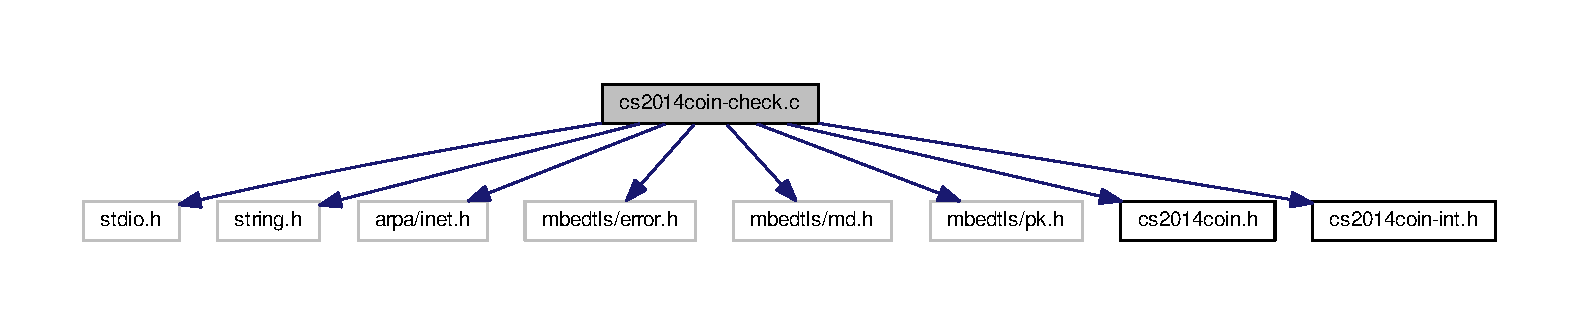
\includegraphics[width=350pt]{cs2014coin-check_8c__incl}
\end{center}
\end{figure}
\subsection*{Macros}
\begin{DoxyCompactItemize}
\item 
\mbox{\Hypertarget{cs2014coin-check_8c_ae24a8f3306fdaad53c6ac0fd494e3d5c}\label{cs2014coin-check_8c_ae24a8f3306fdaad53c6ac0fd494e3d5c}} 
\#define \hyperlink{cs2014coin-check_8c_ae24a8f3306fdaad53c6ac0fd494e3d5c}{SB}(\+\_\+\+\_\+\+\_\+var\+\_\+\+\_\+\+\_\+,  \+\_\+\+\_\+\+\_\+shift\+\_\+\+\_\+\+\_\+)~(\+\_\+\+\_\+\+\_\+var\+\_\+\+\_\+\+\_\+$\vert$=(1$<$$<$\+\_\+\+\_\+\+\_\+shift\+\_\+\+\_\+\+\_\+))
\begin{DoxyCompactList}\small\item\em set a bit in a mask to indicate some error \end{DoxyCompactList}\item 
\mbox{\Hypertarget{cs2014coin-check_8c_a21155e3c6dc04da3b8c6f635e8bf79b8}\label{cs2014coin-check_8c_a21155e3c6dc04da3b8c6f635e8bf79b8}} 
\#define \hyperlink{cs2014coin-check_8c_a21155e3c6dc04da3b8c6f635e8bf79b8}{CB}(\+\_\+\+\_\+\+\_\+var\+\_\+\+\_\+\+\_\+,  \+\_\+\+\_\+\+\_\+shift\+\_\+\+\_\+\+\_\+)~(\+\_\+\+\_\+\+\_\+var\+\_\+\+\_\+\+\_\+\&=$\sim$(1$<$$<$\+\_\+\+\_\+\+\_\+shift\+\_\+\+\_\+\+\_\+))
\begin{DoxyCompactList}\small\item\em clear a bit in a mask to indicate that error wasn\textquotesingle{}t seen \end{DoxyCompactList}\end{DoxyCompactItemize}
\subsection*{Functions}
\begin{DoxyCompactItemize}
\item 
int \hyperlink{cs2014coin-check_8c_a14bef37cd5f67358cd43ce1308049667}{lc\+\_\+memcmp} (const void $\ast$a, const void $\ast$b, size\+\_\+t size)
\begin{DoxyCompactList}\small\item\em a local constant time memcmp \end{DoxyCompactList}\item 
int \hyperlink{cs2014coin-check_8c_ae7d692031170a392c66b9810c65a79a3}{cs2014coin\+\_\+check} (int bits, unsigned char $\ast$buf, int buflen, int $\ast$res)
\begin{DoxyCompactList}\small\item\em check a coin \end{DoxyCompactList}\end{DoxyCompactItemize}


\subsection{Detailed Description}
This is the implemetation of the cs2014 coin checker. 

It should go without saying that these coins are for play\+:-\/)

This is part of C\+S2014 \href{https://down.dsg.cs.tcd.ie/cs2014/examples/c-progs-2/README.html}{\tt https\+://down.\+dsg.\+cs.\+tcd.\+ie/cs2014/examples/c-\/progs-\/2/\+R\+E\+A\+D\+M\+E.\+html} 

\subsection{Function Documentation}
\mbox{\Hypertarget{cs2014coin-check_8c_ae7d692031170a392c66b9810c65a79a3}\label{cs2014coin-check_8c_ae7d692031170a392c66b9810c65a79a3}} 
\index{cs2014coin-\/check.\+c@{cs2014coin-\/check.\+c}!cs2014coin\+\_\+check@{cs2014coin\+\_\+check}}
\index{cs2014coin\+\_\+check@{cs2014coin\+\_\+check}!cs2014coin-\/check.\+c@{cs2014coin-\/check.\+c}}
\subsubsection{\texorpdfstring{cs2014coin\+\_\+check()}{cs2014coin\_check()}}
{\footnotesize\ttfamily int cs2014coin\+\_\+check (\begin{DoxyParamCaption}\item[{int}]{bits,  }\item[{unsigned char $\ast$}]{buf,  }\item[{int}]{buflen,  }\item[{int $\ast$}]{res }\end{DoxyParamCaption})}



check a coin 


\begin{DoxyParams}{Parameters}
{\em bits} & specifies how many bits need to be zero in the hash-\/output \\
\hline
{\em buf} & is an allocated buffer for the coin \\
\hline
{\em buflen} & specifies the input coin size \\
\hline
{\em res} & contains the result of checking the coin \\
\hline
\end{DoxyParams}
\begin{DoxyReturn}{Returns}
zero for success, non-\/zero for fail (note\+: success != good coin!)
\end{DoxyReturn}
Check a coin of the required quality/strength Note we attempt to be roughly constant time here, just for fun But, if this were called on recovered plaintext, that might be significant! See \href{https://cryptocoding.net/index.php/Coding_rules}{\tt https\+://cryptocoding.\+net/index.\+php/\+Coding\+\_\+rules} T\+O\+DO\+: have a dummy public key ready for this so we do sig check of some sort \mbox{\Hypertarget{cs2014coin-check_8c_a14bef37cd5f67358cd43ce1308049667}\label{cs2014coin-check_8c_a14bef37cd5f67358cd43ce1308049667}} 
\index{cs2014coin-\/check.\+c@{cs2014coin-\/check.\+c}!lc\+\_\+memcmp@{lc\+\_\+memcmp}}
\index{lc\+\_\+memcmp@{lc\+\_\+memcmp}!cs2014coin-\/check.\+c@{cs2014coin-\/check.\+c}}
\subsubsection{\texorpdfstring{lc\+\_\+memcmp()}{lc\_memcmp()}}
{\footnotesize\ttfamily int lc\+\_\+memcmp (\begin{DoxyParamCaption}\item[{const void $\ast$}]{a,  }\item[{const void $\ast$}]{b,  }\item[{size\+\_\+t}]{size }\end{DoxyParamCaption})}



a local constant time memcmp 


\begin{DoxyParams}{Parameters}
{\em a} & is buffer 1 \\
\hline
{\em b} & is buffer 2 \\
\hline
{\em size} & is the length of both \\
\hline
\end{DoxyParams}
\begin{DoxyReturn}{Returns}
0 for same, 1 for not same
\end{DoxyReturn}
A constant time memcmp, found at\+: \href{https://github.com/OpenVPN/openvpn/commit/11d21349a4e7e38a025849479b36ace7c2eec2ee}{\tt https\+://github.\+com/\+Open\+V\+P\+N/openvpn/commit/11d21349a4e7e38a025849479b36ace7c2eec2ee} Note -\/ this was done due to a real attck on Open\+V\+PN \href{https://www.rapid7.com/db/vulnerabilities/alpine-linux-cve-2013-2061}{\tt https\+://www.\+rapid7.\+com/db/vulnerabilities/alpine-\/linux-\/cve-\/2013-\/2061} 
\hypertarget{cs2014coin-int_8h}{}\section{cs2014coin-\/int.h File Reference}
\label{cs2014coin-int_8h}\index{cs2014coin-\/int.\+h@{cs2014coin-\/int.\+h}}


Definitions/macros used internally.  


This graph shows which files directly or indirectly include this file\+:\nopagebreak
\begin{figure}[H]
\begin{center}
\leavevmode
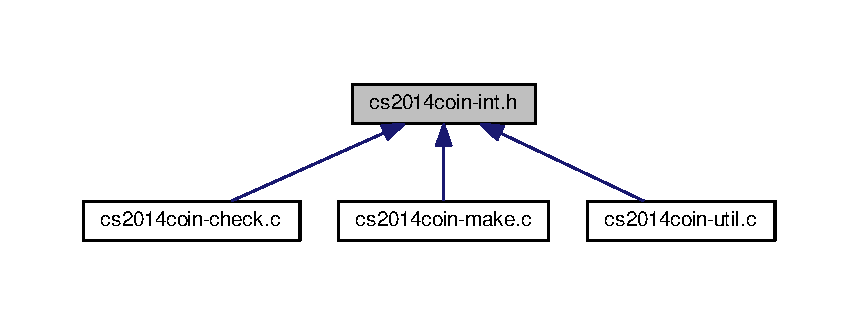
\includegraphics[width=350pt]{cs2014coin-int_8h__dep__incl}
\end{center}
\end{figure}
\subsection*{Macros}
\begin{DoxyCompactItemize}
\item 
\mbox{\Hypertarget{cs2014coin-int_8h_a0f085055294117dfcbd472c7822b0e23}\label{cs2014coin-int_8h_a0f085055294117dfcbd472c7822b0e23}} 
\#define \hyperlink{cs2014coin-int_8h_a0f085055294117dfcbd472c7822b0e23}{C\+C\+\_\+\+B\+U\+F\+S\+IZ}~16000
\begin{DoxyCompactList}\small\item\em we\textquotesingle{}ll use this on stack to save coding mallocs etc \end{DoxyCompactList}\item 
\mbox{\Hypertarget{cs2014coin-int_8h_a1a3f34ffaae00f1c83da9a7c63170cb0}\label{cs2014coin-int_8h_a1a3f34ffaae00f1c83da9a7c63170cb0}} 
\#define \hyperlink{cs2014coin-int_8h_a1a3f34ffaae00f1c83da9a7c63170cb0}{C\+C\+\_\+\+D\+E\+F\+E\+RR}~\char`\"{}Bummer, no idea what went wrong there\char`\"{}
\begin{DoxyCompactList}\small\item\em a generic error \end{DoxyCompactList}\item 
\mbox{\Hypertarget{cs2014coin-int_8h_a6160fdc571466ec7d48a39c9fc708af3}\label{cs2014coin-int_8h_a6160fdc571466ec7d48a39c9fc708af3}} 
\#define \hyperlink{cs2014coin-int_8h_a6160fdc571466ec7d48a39c9fc708af3}{C\+C\+\_\+\+G\+E\+N\+E\+RR}~\char`\"{}Some kind of fairly generic error happened\char`\"{}
\begin{DoxyCompactList}\small\item\em another generic error \end{DoxyCompactList}\item 
\mbox{\Hypertarget{cs2014coin-int_8h_a3c59fec65b0487d41c9c642ff283f175}\label{cs2014coin-int_8h_a3c59fec65b0487d41c9c642ff283f175}} 
\#define \hyperlink{cs2014coin-int_8h_a3c59fec65b0487d41c9c642ff283f175}{C\+C\+\_\+\+T\+O\+O\+L\+O\+NG}~1
\begin{DoxyCompactList}\small\item\em input is too long \end{DoxyCompactList}\item 
\mbox{\Hypertarget{cs2014coin-int_8h_a3c13d1329b1f863c15fd4b83411c2d95}\label{cs2014coin-int_8h_a3c13d1329b1f863c15fd4b83411c2d95}} 
\#define \hyperlink{cs2014coin-int_8h_a3c13d1329b1f863c15fd4b83411c2d95}{C\+C\+\_\+\+D\+R\+B\+G\+C\+R\+AP}~2
\begin{DoxyCompactList}\small\item\em can\textquotesingle{}t initiate D\+R\+BG \end{DoxyCompactList}\item 
\mbox{\Hypertarget{cs2014coin-int_8h_a38c67b7590b216f386011c1abb1e139c}\label{cs2014coin-int_8h_a38c67b7590b216f386011c1abb1e139c}} 
\#define \hyperlink{cs2014coin-int_8h_a38c67b7590b216f386011c1abb1e139c}{C\+C\+\_\+\+K\+E\+Y\+G\+E\+N\+F\+A\+IL}~3
\begin{DoxyCompactList}\small\item\em key generator failed \end{DoxyCompactList}\item 
\mbox{\Hypertarget{cs2014coin-int_8h_a1147a2a3b8060721af3ae0907a76a50e}\label{cs2014coin-int_8h_a1147a2a3b8060721af3ae0907a76a50e}} 
\#define \hyperlink{cs2014coin-int_8h_a1147a2a3b8060721af3ae0907a76a50e}{C\+C\+\_\+\+I\+T\+E\+RS}~4
\begin{DoxyCompactList}\small\item\em an error to use if we\textquotesingle{}ve iterated too much searching for a coin \end{DoxyCompactList}\item 
\mbox{\Hypertarget{cs2014coin-int_8h_a3ed3e314f0241fad2ac2379da85b8c70}\label{cs2014coin-int_8h_a3ed3e314f0241fad2ac2379da85b8c70}} 
\#define \hyperlink{cs2014coin-int_8h_a3ed3e314f0241fad2ac2379da85b8c70}{C\+C\+\_\+\+B\+A\+D\+C\+I\+P\+H\+E\+R\+S\+U\+I\+TE}~5
\begin{DoxyCompactList}\small\item\em an unknown ciphersuite \end{DoxyCompactList}\item 
\#define \hyperlink{cs2014coin-int_8h_a0f02326e76cf787367d95020eac57531}{N\+O\+\_\+\+C\+C\+\_\+\+D\+E\+B\+UG}
\begin{DoxyCompactList}\small\item\em turns off debug printing \end{DoxyCompactList}\item 
\#define \hyperlink{cs2014coin-int_8h_afa38166e59791a080ff9c3096c84146a}{N\+O\+\_\+\+C\+C\+\_\+\+D\+E\+B\+U\+G\+\_\+\+E\+X\+T\+RA}
\begin{DoxyCompactList}\small\item\em turns off loadsa debugging \end{DoxyCompactList}\end{DoxyCompactItemize}
\subsection*{Functions}
\begin{DoxyCompactItemize}
\item 
void \hyperlink{cs2014coin-int_8h_afd151090a1b9f8e9a800daa05be4bbf6}{dumpbuf} (char $\ast$msg, unsigned char $\ast$buffer, int buflen)
\begin{DoxyCompactList}\small\item\em debug printer for buffers \end{DoxyCompactList}\item 
int \hyperlink{cs2014coin-int_8h_a703c5c765e9038368f07fa48d3a89934}{zero\+\_\+bits} (int bits, unsigned char $\ast$buf, int buflen)
\begin{DoxyCompactList}\small\item\em check if rightmost N bits of a buffer are zero \end{DoxyCompactList}\end{DoxyCompactItemize}
\subsection*{Variables}
\begin{DoxyCompactItemize}
\item 
const char $\ast$ \hyperlink{cs2014coin-int_8h_a8e3da0eb987e1e7cd239012fe8d18655}{errstrs} \mbox{[}$\,$\mbox{]}
\begin{DoxyCompactList}\small\item\em an array of speciic strings -\/ C\+C\+\_\+foo \#define\textquotesingle{}d values are index the strings in this array \end{DoxyCompactList}\end{DoxyCompactItemize}


\subsection{Detailed Description}
Definitions/macros used internally. 

It should go without saying that these coins are for play\+:-\/)

This is part of C\+S2014 \href{https://down.dsg.cs.tcd.ie/cs2014/examples/c-progs-2/README.html}{\tt https\+://down.\+dsg.\+cs.\+tcd.\+ie/cs2014/examples/c-\/progs-\/2/\+R\+E\+A\+D\+M\+E.\+html} 

\subsection{Macro Definition Documentation}
\mbox{\Hypertarget{cs2014coin-int_8h_a0f02326e76cf787367d95020eac57531}\label{cs2014coin-int_8h_a0f02326e76cf787367d95020eac57531}} 
\index{cs2014coin-\/int.\+h@{cs2014coin-\/int.\+h}!N\+O\+\_\+\+C\+C\+\_\+\+D\+E\+B\+UG@{N\+O\+\_\+\+C\+C\+\_\+\+D\+E\+B\+UG}}
\index{N\+O\+\_\+\+C\+C\+\_\+\+D\+E\+B\+UG@{N\+O\+\_\+\+C\+C\+\_\+\+D\+E\+B\+UG}!cs2014coin-\/int.\+h@{cs2014coin-\/int.\+h}}
\subsubsection{\texorpdfstring{N\+O\+\_\+\+C\+C\+\_\+\+D\+E\+B\+UG}{NO\_CC\_DEBUG}}
{\footnotesize\ttfamily \#define N\+O\+\_\+\+C\+C\+\_\+\+D\+E\+B\+UG}



turns off debug printing 

this form of macro is only there to keep doxygen happy what we (normally) want is to undef C\+C\+\_\+\+D\+E\+B\+UG, but the bare under confuses doxygenturns on some debug printing \mbox{\Hypertarget{cs2014coin-int_8h_afa38166e59791a080ff9c3096c84146a}\label{cs2014coin-int_8h_afa38166e59791a080ff9c3096c84146a}} 
\index{cs2014coin-\/int.\+h@{cs2014coin-\/int.\+h}!N\+O\+\_\+\+C\+C\+\_\+\+D\+E\+B\+U\+G\+\_\+\+E\+X\+T\+RA@{N\+O\+\_\+\+C\+C\+\_\+\+D\+E\+B\+U\+G\+\_\+\+E\+X\+T\+RA}}
\index{N\+O\+\_\+\+C\+C\+\_\+\+D\+E\+B\+U\+G\+\_\+\+E\+X\+T\+RA@{N\+O\+\_\+\+C\+C\+\_\+\+D\+E\+B\+U\+G\+\_\+\+E\+X\+T\+RA}!cs2014coin-\/int.\+h@{cs2014coin-\/int.\+h}}
\subsubsection{\texorpdfstring{N\+O\+\_\+\+C\+C\+\_\+\+D\+E\+B\+U\+G\+\_\+\+E\+X\+T\+RA}{NO\_CC\_DEBUG\_EXTRA}}
{\footnotesize\ttfamily \#define N\+O\+\_\+\+C\+C\+\_\+\+D\+E\+B\+U\+G\+\_\+\+E\+X\+T\+RA}



turns off loadsa debugging 

this form of macro is only there to keep doxygen happy what we (normally) want is to undef C\+C\+\_\+\+D\+E\+B\+U\+G\+\_\+\+E\+X\+T\+RA, but the bare under confuses doxygenturns on loadsa debugging 

\subsection{Function Documentation}
\mbox{\Hypertarget{cs2014coin-int_8h_afd151090a1b9f8e9a800daa05be4bbf6}\label{cs2014coin-int_8h_afd151090a1b9f8e9a800daa05be4bbf6}} 
\index{cs2014coin-\/int.\+h@{cs2014coin-\/int.\+h}!dumpbuf@{dumpbuf}}
\index{dumpbuf@{dumpbuf}!cs2014coin-\/int.\+h@{cs2014coin-\/int.\+h}}
\subsubsection{\texorpdfstring{dumpbuf()}{dumpbuf()}}
{\footnotesize\ttfamily void dumpbuf (\begin{DoxyParamCaption}\item[{char $\ast$}]{msg,  }\item[{unsigned char $\ast$}]{buffer,  }\item[{int}]{buflen }\end{DoxyParamCaption})}



debug printer for buffers 


\begin{DoxyParams}{Parameters}
{\em buffer} & is where stuff\textquotesingle{}s at  buflen is how many octets \\
\hline
\end{DoxyParams}
\begin{DoxyReturn}{Returns}
void
\end{DoxyReturn}
debug printer for buffers


\begin{DoxyParams}{Parameters}
{\em buffer} & is where stuff\textquotesingle{}s at  buflen is how many octets \\
\hline
\end{DoxyParams}
\begin{DoxyReturn}{Returns}
void 
\end{DoxyReturn}
\mbox{\Hypertarget{cs2014coin-int_8h_a703c5c765e9038368f07fa48d3a89934}\label{cs2014coin-int_8h_a703c5c765e9038368f07fa48d3a89934}} 
\index{cs2014coin-\/int.\+h@{cs2014coin-\/int.\+h}!zero\+\_\+bits@{zero\+\_\+bits}}
\index{zero\+\_\+bits@{zero\+\_\+bits}!cs2014coin-\/int.\+h@{cs2014coin-\/int.\+h}}
\subsubsection{\texorpdfstring{zero\+\_\+bits()}{zero\_bits()}}
{\footnotesize\ttfamily int zero\+\_\+bits (\begin{DoxyParamCaption}\item[{int}]{bits,  }\item[{unsigned char $\ast$}]{buf,  }\item[{int}]{buflen }\end{DoxyParamCaption})}



check if rightmost N bits of a buffer are zero 


\begin{DoxyParams}{Parameters}
{\em bits} & is the value of N (in bits) \\
\hline
{\em buf} & is the buffer \\
\hline
{\em buflen} & is the length \\
\hline
\end{DoxyParams}
\begin{DoxyReturn}{Returns}
1 if those N bits are all zero, 0 otherwise
\end{DoxyReturn}
be better if this were more efficient


\begin{DoxyParams}{Parameters}
{\em bits} & is the value of N (in bits) \\
\hline
{\em buf} & is the buffer \\
\hline
{\em buflen} & is the length \\
\hline
\end{DoxyParams}
\begin{DoxyReturn}{Returns}
1 if those N bits are all zero, 0 otherwise
\end{DoxyReturn}
be better if this were more efficient also be better if this were constant time so in real-\/world code we ought probably have two versions of this one, for coin checking that\textquotesingle{}s constant time, but doesn\textquotesingle{}t need to be too efficient and one for mining that doesn\textquotesingle{}t need to be constant time but does need max efficiency 

\subsection{Variable Documentation}
\mbox{\Hypertarget{cs2014coin-int_8h_a8e3da0eb987e1e7cd239012fe8d18655}\label{cs2014coin-int_8h_a8e3da0eb987e1e7cd239012fe8d18655}} 
\index{cs2014coin-\/int.\+h@{cs2014coin-\/int.\+h}!errstrs@{errstrs}}
\index{errstrs@{errstrs}!cs2014coin-\/int.\+h@{cs2014coin-\/int.\+h}}
\subsubsection{\texorpdfstring{errstrs}{errstrs}}
{\footnotesize\ttfamily const char$\ast$ errstrs\mbox{[}$\,$\mbox{]}}



an array of speciic strings -\/ C\+C\+\_\+foo \#define\textquotesingle{}d values are index the strings in this array 

an array of speciic strings -\/ C\+C\+\_\+foo \#define\textquotesingle{}d values are index the strings in this array 
\hypertarget{cs2014coin-main_8c}{}\section{cs2014coin-\/main.c File Reference}
\label{cs2014coin-main_8c}\index{cs2014coin-\/main.\+c@{cs2014coin-\/main.\+c}}


This is the main function for cs2014 coin handling.  


{\ttfamily \#include $<$stdio.\+h$>$}\newline
{\ttfamily \#include $<$stdlib.\+h$>$}\newline
{\ttfamily \#include $<$string.\+h$>$}\newline
{\ttfamily \#include $<$getopt.\+h$>$}\newline
{\ttfamily \#include \char`\"{}cs2014coin.\+h\char`\"{}}\newline
Include dependency graph for cs2014coin-\/main.c\+:\nopagebreak
\begin{figure}[H]
\begin{center}
\leavevmode
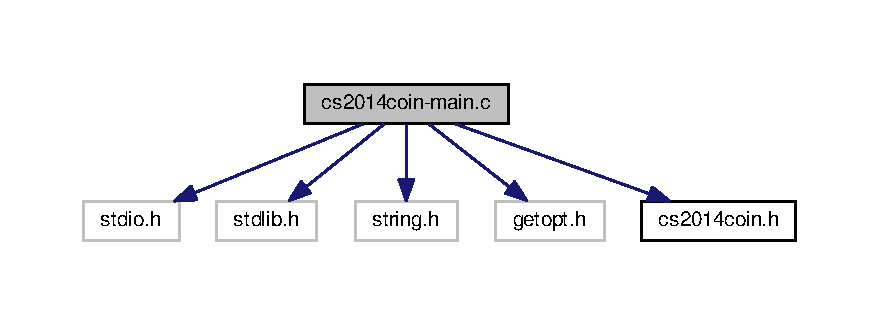
\includegraphics[width=350pt]{cs2014coin-main_8c__incl}
\end{center}
\end{figure}
\subsection*{Macros}
\begin{DoxyCompactItemize}
\item 
\#define \hyperlink{cs2014coin-main_8c_a27a1bcd135235e6fd1b52af23cb7886a}{M\+A\+X\+Z\+E\+R\+O\+B\+I\+TS}~20
\begin{DoxyCompactList}\small\item\em the A\+PI we want... \end{DoxyCompactList}\item 
\mbox{\Hypertarget{cs2014coin-main_8c_a7405332bf1fd750e532b1e333cf41092}\label{cs2014coin-main_8c_a7405332bf1fd750e532b1e333cf41092}} 
\#define \hyperlink{cs2014coin-main_8c_a7405332bf1fd750e532b1e333cf41092}{D\+E\+F\+Z\+E\+R\+O\+B\+I\+TS}~17
\begin{DoxyCompactList}\small\item\em the default length of zero-\/bit run \end{DoxyCompactList}\item 
\mbox{\Hypertarget{cs2014coin-main_8c_aca6b7654301c81946540a3f80694b140}\label{cs2014coin-main_8c_aca6b7654301c81946540a3f80694b140}} 
\#define \hyperlink{cs2014coin-main_8c_aca6b7654301c81946540a3f80694b140}{M\+O\+D\+E\+\_\+\+M\+A\+KE}~0
\begin{DoxyCompactList}\small\item\em mode where we make a coin \end{DoxyCompactList}\item 
\mbox{\Hypertarget{cs2014coin-main_8c_a04b254126af7e934b608d6fc4f570518}\label{cs2014coin-main_8c_a04b254126af7e934b608d6fc4f570518}} 
\#define \hyperlink{cs2014coin-main_8c_a04b254126af7e934b608d6fc4f570518}{M\+O\+D\+E\+\_\+\+C\+H\+E\+CK}~1
\begin{DoxyCompactList}\small\item\em mode where we check a coin looks feasible \end{DoxyCompactList}\item 
\mbox{\Hypertarget{cs2014coin-main_8c_ad3abbe096450034083770ac55806d999}\label{cs2014coin-main_8c_ad3abbe096450034083770ac55806d999}} 
\#define \hyperlink{cs2014coin-main_8c_ad3abbe096450034083770ac55806d999}{D\+E\+F\+F\+N\+A\+ME}~\char`\"{}cs2014.\+coin\char`\"{}
\begin{DoxyCompactList}\small\item\em default file name \end{DoxyCompactList}\end{DoxyCompactItemize}
\subsection*{Functions}
\begin{DoxyCompactItemize}
\item 
\mbox{\Hypertarget{cs2014coin-main_8c_a9a05fb05f758a87628212c4bfc50c182}\label{cs2014coin-main_8c_a9a05fb05f758a87628212c4bfc50c182}} 
void {\bfseries usage} (char $\ast$progname)
\item 
int \hyperlink{cs2014coin-main_8c_a0ddf1224851353fc92bfbff6f499fa97}{main} (int argc, char $\ast$argv\mbox{[}$\,$\mbox{]})
\end{DoxyCompactItemize}


\subsection{Detailed Description}
This is the main function for cs2014 coin handling. 

This is part of C\+S2014 \href{https://down.dsg.cs.tcd.ie/cs2014/examples/c-progs-2/README.html}{\tt https\+://down.\+dsg.\+cs.\+tcd.\+ie/cs2014/examples/c-\/progs-\/2/\+R\+E\+A\+D\+M\+E.\+html} 

\subsection{Macro Definition Documentation}
\mbox{\Hypertarget{cs2014coin-main_8c_a27a1bcd135235e6fd1b52af23cb7886a}\label{cs2014coin-main_8c_a27a1bcd135235e6fd1b52af23cb7886a}} 
\index{cs2014coin-\/main.\+c@{cs2014coin-\/main.\+c}!M\+A\+X\+Z\+E\+R\+O\+B\+I\+TS@{M\+A\+X\+Z\+E\+R\+O\+B\+I\+TS}}
\index{M\+A\+X\+Z\+E\+R\+O\+B\+I\+TS@{M\+A\+X\+Z\+E\+R\+O\+B\+I\+TS}!cs2014coin-\/main.\+c@{cs2014coin-\/main.\+c}}
\subsubsection{\texorpdfstring{M\+A\+X\+Z\+E\+R\+O\+B\+I\+TS}{MAXZEROBITS}}
{\footnotesize\ttfamily \#define M\+A\+X\+Z\+E\+R\+O\+B\+I\+TS~20}



the A\+PI we want... 

the max length of zero-\/bit run we can support 

\subsection{Function Documentation}
\mbox{\Hypertarget{cs2014coin-main_8c_a0ddf1224851353fc92bfbff6f499fa97}\label{cs2014coin-main_8c_a0ddf1224851353fc92bfbff6f499fa97}} 
\index{cs2014coin-\/main.\+c@{cs2014coin-\/main.\+c}!main@{main}}
\index{main@{main}!cs2014coin-\/main.\+c@{cs2014coin-\/main.\+c}}
\subsubsection{\texorpdfstring{main()}{main()}}
{\footnotesize\ttfamily int main (\begin{DoxyParamCaption}\item[{int}]{argc,  }\item[{char $\ast$}]{argv\mbox{[}$\,$\mbox{]} }\end{DoxyParamCaption})}

buffer for a coin

string for file name 
\hypertarget{cs2014coin-make_8c}{}\section{cs2014coin-\/make.c File Reference}
\label{cs2014coin-make_8c}\index{cs2014coin-\/make.\+c@{cs2014coin-\/make.\+c}}


This is the implementation of the cs2014 coin maker.  


{\ttfamily \#include $<$stdio.\+h$>$}\newline
{\ttfamily \#include $<$string.\+h$>$}\newline
{\ttfamily \#include \char`\"{}cs2014coin.\+h\char`\"{}}\newline
{\ttfamily \#include \char`\"{}cs2014coin-\/int.\+h\char`\"{}}\newline
Include dependency graph for cs2014coin-\/make.c\+:\nopagebreak
\begin{figure}[H]
\begin{center}
\leavevmode
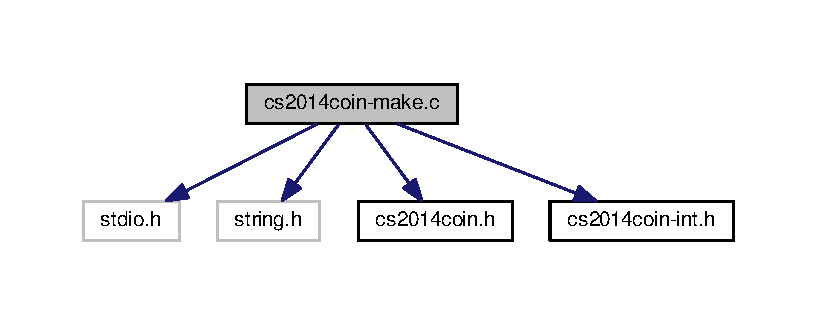
\includegraphics[width=350pt]{cs2014coin-make_8c__incl}
\end{center}
\end{figure}
\subsection*{Functions}
\begin{DoxyCompactItemize}
\item 
int \hyperlink{cs2014coin-make_8c_a71eabb5a75b43b92f05f52bff713e429}{cs2014coin\+\_\+make} (int bits, unsigned char $\ast$buf, int $\ast$buflen)
\begin{DoxyCompactList}\small\item\em make a coin \end{DoxyCompactList}\end{DoxyCompactItemize}


\subsection{Detailed Description}
This is the implementation of the cs2014 coin maker. 

It should go without saying that these coins are for play\+:-\/)

This is part of C\+S2014 \href{https://down.dsg.cs.tcd.ie/cs2014/examples/c-progs-2/README.html}{\tt https\+://down.\+dsg.\+cs.\+tcd.\+ie/cs2014/examples/c-\/progs-\/2/\+R\+E\+A\+D\+M\+E.\+html} 

\subsection{Function Documentation}
\mbox{\Hypertarget{cs2014coin-make_8c_a71eabb5a75b43b92f05f52bff713e429}\label{cs2014coin-make_8c_a71eabb5a75b43b92f05f52bff713e429}} 
\index{cs2014coin-\/make.\+c@{cs2014coin-\/make.\+c}!cs2014coin\+\_\+make@{cs2014coin\+\_\+make}}
\index{cs2014coin\+\_\+make@{cs2014coin\+\_\+make}!cs2014coin-\/make.\+c@{cs2014coin-\/make.\+c}}
\subsubsection{\texorpdfstring{cs2014coin\+\_\+make()}{cs2014coin\_make()}}
{\footnotesize\ttfamily int cs2014coin\+\_\+make (\begin{DoxyParamCaption}\item[{int}]{bits,  }\item[{unsigned char $\ast$}]{buf,  }\item[{int $\ast$}]{buflen }\end{DoxyParamCaption})}



make a coin 


\begin{DoxyParams}{Parameters}
{\em bits} & specifies how many bits need to be zero in the hash-\/output \\
\hline
{\em buf} & is an allocated buffer for the coin \\
\hline
{\em buflen} & is an in/out parameter reflecting the buffer-\/size/actual-\/coin-\/size \\
\hline
\end{DoxyParams}
\begin{DoxyReturn}{Returns}
zero for success, non-\/zero for fail
\end{DoxyReturn}
Make me a coin of the required quality/strength 
\hypertarget{cs2014coin-util_8c}{}\section{cs2014coin-\/util.c File Reference}
\label{cs2014coin-util_8c}\index{cs2014coin-\/util.\+c@{cs2014coin-\/util.\+c}}


This is the implementation of utilities for cs2014 coins.  


{\ttfamily \#include $<$stdio.\+h$>$}\newline
{\ttfamily \#include \char`\"{}cs2014coin.\+h\char`\"{}}\newline
{\ttfamily \#include \char`\"{}cs2014coin-\/int.\+h\char`\"{}}\newline
Include dependency graph for cs2014coin-\/util.c\+:\nopagebreak
\begin{figure}[H]
\begin{center}
\leavevmode
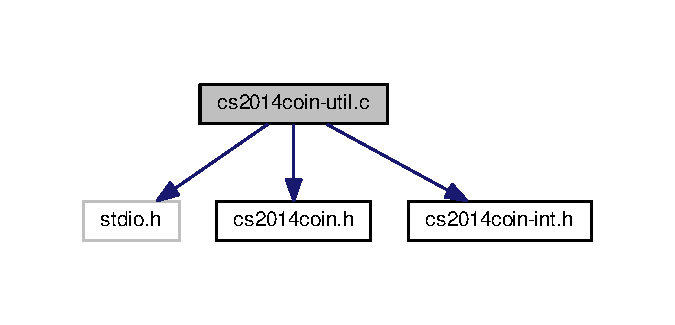
\includegraphics[width=324pt]{cs2014coin-util_8c__incl}
\end{center}
\end{figure}
\subsection*{Macros}
\begin{DoxyCompactItemize}
\item 
\mbox{\Hypertarget{cs2014coin-util_8c_a83079f604f51143b0e11495d30d58b20}\label{cs2014coin-util_8c_a83079f604f51143b0e11495d30d58b20}} 
\#define \hyperlink{cs2014coin-util_8c_a83079f604f51143b0e11495d30d58b20}{C\+C\+\_\+\+M\+A\+X\+E\+RR}~(sizeof(\hyperlink{cs2014coin-util_8c_a8e3da0eb987e1e7cd239012fe8d18655}{errstrs})/sizeof(const char$\ast$))
\begin{DoxyCompactList}\small\item\em macro for how many errors we have \end{DoxyCompactList}\end{DoxyCompactItemize}
\subsection*{Functions}
\begin{DoxyCompactItemize}
\item 
const char $\ast$ \hyperlink{cs2014coin-util_8c_af955b20ed8c88563e864ecca0b2e538e}{cs2014coin\+\_\+err} (int errno)
\begin{DoxyCompactList}\small\item\em return out best guess error string \end{DoxyCompactList}\item 
void \hyperlink{cs2014coin-util_8c_afd151090a1b9f8e9a800daa05be4bbf6}{dumpbuf} (char $\ast$msg, unsigned char $\ast$buffer, int buflen)
\begin{DoxyCompactList}\small\item\em debug printerfor buffers \end{DoxyCompactList}\item 
int \hyperlink{cs2014coin-util_8c_a703c5c765e9038368f07fa48d3a89934}{zero\+\_\+bits} (int bits, unsigned char $\ast$buf, int buflen)
\begin{DoxyCompactList}\small\item\em check if rightmost N bits of a buffer are zero \end{DoxyCompactList}\end{DoxyCompactItemize}
\subsection*{Variables}
\begin{DoxyCompactItemize}
\item 
const char $\ast$ \hyperlink{cs2014coin-util_8c_a8e3da0eb987e1e7cd239012fe8d18655}{errstrs} \mbox{[}$\,$\mbox{]}
\begin{DoxyCompactList}\small\item\em an array of speciic strings \end{DoxyCompactList}\end{DoxyCompactItemize}


\subsection{Detailed Description}
This is the implementation of utilities for cs2014 coins. 

It should go without saying that these coins are for play\+:-\/)

This is part of C\+S2014 \href{https://down.dsg.cs.tcd.ie/cs2014/examples/c-progs-2/README.html}{\tt https\+://down.\+dsg.\+cs.\+tcd.\+ie/cs2014/examples/c-\/progs-\/2/\+R\+E\+A\+D\+M\+E.\+html} 

\subsection{Function Documentation}
\mbox{\Hypertarget{cs2014coin-util_8c_af955b20ed8c88563e864ecca0b2e538e}\label{cs2014coin-util_8c_af955b20ed8c88563e864ecca0b2e538e}} 
\index{cs2014coin-\/util.\+c@{cs2014coin-\/util.\+c}!cs2014coin\+\_\+err@{cs2014coin\+\_\+err}}
\index{cs2014coin\+\_\+err@{cs2014coin\+\_\+err}!cs2014coin-\/util.\+c@{cs2014coin-\/util.\+c}}
\subsubsection{\texorpdfstring{cs2014coin\+\_\+err()}{cs2014coin\_err()}}
{\footnotesize\ttfamily const char$\ast$ cs2014coin\+\_\+err (\begin{DoxyParamCaption}\item[{int}]{errno }\end{DoxyParamCaption})}



return out best guess error string 


\begin{DoxyParams}{Parameters}
{\em errno} & is an errno, presumably returned from somewhere else in this A\+PI \\
\hline
\end{DoxyParams}
\begin{DoxyReturn}{Returns}
error string (a const)
\end{DoxyReturn}
Error string handler. Good to use unique error numbers for all different conditions \mbox{\Hypertarget{cs2014coin-util_8c_afd151090a1b9f8e9a800daa05be4bbf6}\label{cs2014coin-util_8c_afd151090a1b9f8e9a800daa05be4bbf6}} 
\index{cs2014coin-\/util.\+c@{cs2014coin-\/util.\+c}!dumpbuf@{dumpbuf}}
\index{dumpbuf@{dumpbuf}!cs2014coin-\/util.\+c@{cs2014coin-\/util.\+c}}
\subsubsection{\texorpdfstring{dumpbuf()}{dumpbuf()}}
{\footnotesize\ttfamily void dumpbuf (\begin{DoxyParamCaption}\item[{char $\ast$}]{msg,  }\item[{unsigned char $\ast$}]{buffer,  }\item[{int}]{buflen }\end{DoxyParamCaption})}



debug printerfor buffers 

debug printer for buffers


\begin{DoxyParams}{Parameters}
{\em buffer} & is where stuff\textquotesingle{}s at  buflen is how many octets \\
\hline
\end{DoxyParams}
\begin{DoxyReturn}{Returns}
void 
\end{DoxyReturn}
\mbox{\Hypertarget{cs2014coin-util_8c_a703c5c765e9038368f07fa48d3a89934}\label{cs2014coin-util_8c_a703c5c765e9038368f07fa48d3a89934}} 
\index{cs2014coin-\/util.\+c@{cs2014coin-\/util.\+c}!zero\+\_\+bits@{zero\+\_\+bits}}
\index{zero\+\_\+bits@{zero\+\_\+bits}!cs2014coin-\/util.\+c@{cs2014coin-\/util.\+c}}
\subsubsection{\texorpdfstring{zero\+\_\+bits()}{zero\_bits()}}
{\footnotesize\ttfamily int zero\+\_\+bits (\begin{DoxyParamCaption}\item[{int}]{bits,  }\item[{unsigned char $\ast$}]{buf,  }\item[{int}]{buflen }\end{DoxyParamCaption})}



check if rightmost N bits of a buffer are zero 


\begin{DoxyParams}{Parameters}
{\em bits} & is the value of N (in bits) \\
\hline
{\em buf} & is the buffer \\
\hline
{\em buflen} & is the length \\
\hline
\end{DoxyParams}
\begin{DoxyReturn}{Returns}
1 if those N bits are all zero, 0 otherwise
\end{DoxyReturn}
be better if this were more efficient also be better if this were constant time so in real-\/world code we ought probably have two versions of this one, for coin checking that\textquotesingle{}s constant time, but doesn\textquotesingle{}t need to be too efficient and one for mining that doesn\textquotesingle{}t need to be constant time but does need max efficiency 

\subsection{Variable Documentation}
\mbox{\Hypertarget{cs2014coin-util_8c_a8e3da0eb987e1e7cd239012fe8d18655}\label{cs2014coin-util_8c_a8e3da0eb987e1e7cd239012fe8d18655}} 
\index{cs2014coin-\/util.\+c@{cs2014coin-\/util.\+c}!errstrs@{errstrs}}
\index{errstrs@{errstrs}!cs2014coin-\/util.\+c@{cs2014coin-\/util.\+c}}
\subsubsection{\texorpdfstring{errstrs}{errstrs}}
{\footnotesize\ttfamily const char$\ast$ errstrs\mbox{[}$\,$\mbox{]}}

{\bfseries Initial value\+:}
\begin{DoxyCode}
=\{
\textcolor{stringliteral}{"This should never be seen"},
\textcolor{stringliteral}{"That's a mad length"},
\textcolor{stringliteral}{"DRBG failed, which is odd"},
\textcolor{stringliteral}{"Key generator failed, which is very odd"},
\textcolor{stringliteral}{"Too many iterations, sorry"},
\textcolor{stringliteral}{"Unknown ciphersuite"},
\}
\end{DoxyCode}


an array of speciic strings 

an array of speciic strings -\/ C\+C\+\_\+foo \#define\textquotesingle{}d values are index the strings in this array 
\hypertarget{cs2014coin_8h}{}\section{cs2014coin.\+h File Reference}
\label{cs2014coin_8h}\index{cs2014coin.\+h@{cs2014coin.\+h}}


This is the external i/f for the cs2014 coin example.  


This graph shows which files directly or indirectly include this file\+:\nopagebreak
\begin{figure}[H]
\begin{center}
\leavevmode
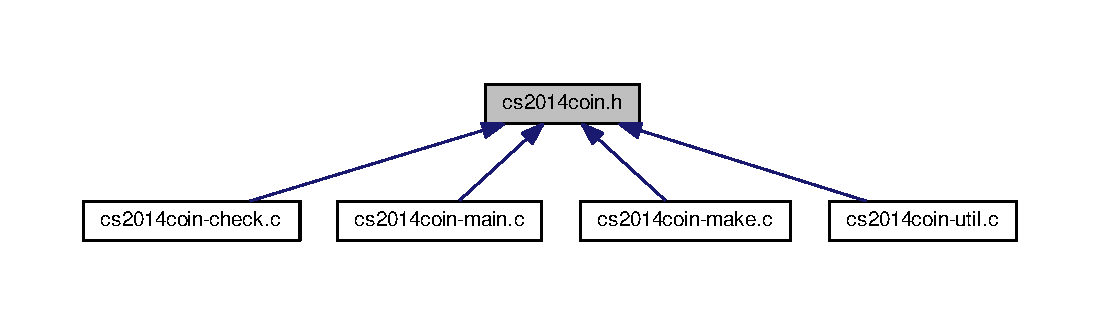
\includegraphics[width=350pt]{cs2014coin_8h__dep__incl}
\end{center}
\end{figure}
\subsection*{Classes}
\begin{DoxyCompactItemize}
\item 
struct \hyperlink{structcs2014coin__t__defn}{cs2014coin\+\_\+t\+\_\+defn}
\begin{DoxyCompactList}\small\item\em our basic cs2094 coin type \end{DoxyCompactList}\end{DoxyCompactItemize}
\subsection*{Macros}
\begin{DoxyCompactItemize}
\item 
\mbox{\Hypertarget{cs2014coin_8h_a8626eb8e0b824c47a00ed9dfb411763c}\label{cs2014coin_8h_a8626eb8e0b824c47a00ed9dfb411763c}} 
\#define {\bfseries C\+S2014\+C\+O\+I\+N\+\_\+\+B\+U\+F\+S\+I\+ZE}~1024
\item 
\mbox{\Hypertarget{cs2014coin_8h_abc0ab920e51b69083b4a29ab8813dd9d}\label{cs2014coin_8h_abc0ab920e51b69083b4a29ab8813dd9d}} 
\#define {\bfseries C\+S2014\+C\+O\+I\+N\+\_\+\+P\+R\+O\+G\+R\+E\+SS}
\item 
\mbox{\Hypertarget{cs2014coin_8h_a960fed81511c80d2f7fc0e7e999a27a7}\label{cs2014coin_8h_a960fed81511c80d2f7fc0e7e999a27a7}} 
\#define {\bfseries C\+S2014\+C\+O\+I\+N\+\_\+\+G\+O\+OD}~0
\item 
\mbox{\Hypertarget{cs2014coin_8h_a2f8ba6442a275cba66d527bb610f4589}\label{cs2014coin_8h_a2f8ba6442a275cba66d527bb610f4589}} 
\#define {\bfseries C\+S2014\+C\+O\+I\+N\+\_\+\+B\+AD}~1
\item 
\mbox{\Hypertarget{cs2014coin_8h_a5364e9ad0c03c30ff9f8ab7a81f52078}\label{cs2014coin_8h_a5364e9ad0c03c30ff9f8ab7a81f52078}} 
\#define {\bfseries C\+S2014\+C\+O\+I\+N\+\_\+\+G\+E\+N\+E\+RR}~-\/1
\item 
\mbox{\Hypertarget{cs2014coin_8h_a20da7173260bf769bcafbb06c7b119b4}\label{cs2014coin_8h_a20da7173260bf769bcafbb06c7b119b4}} 
\#define {\bfseries C\+S2014\+C\+O\+I\+N\+\_\+\+M\+A\+X\+I\+T\+ER}~1024$\ast$1024
\item 
\mbox{\Hypertarget{cs2014coin_8h_a325f4a58f8c9840992edfa4972f90bef}\label{cs2014coin_8h_a325f4a58f8c9840992edfa4972f90bef}} 
\#define {\bfseries C\+S2014\+C\+O\+I\+N\+\_\+\+C\+S\+\_\+0}~0
\end{DoxyCompactItemize}
\subsection*{Typedefs}
\begin{DoxyCompactItemize}
\item 
typedef struct \hyperlink{structcs2014coin__t__defn}{cs2014coin\+\_\+t\+\_\+defn} \hyperlink{cs2014coin_8h_a7ac320e3e2bce433242b9358c51a34c8}{cs2014coin\+\_\+t}
\begin{DoxyCompactList}\small\item\em our basic cs2094 coin type \end{DoxyCompactList}\end{DoxyCompactItemize}
\subsection*{Functions}
\begin{DoxyCompactItemize}
\item 
const char $\ast$ \hyperlink{cs2014coin_8h_af955b20ed8c88563e864ecca0b2e538e}{cs2014coin\+\_\+err} (int errno)
\begin{DoxyCompactList}\small\item\em return out best guess error string \end{DoxyCompactList}\item 
int \hyperlink{cs2014coin_8h_a71eabb5a75b43b92f05f52bff713e429}{cs2014coin\+\_\+make} (int bits, unsigned char $\ast$buf, int $\ast$buflen)
\begin{DoxyCompactList}\small\item\em make a coin \end{DoxyCompactList}\item 
int \hyperlink{cs2014coin_8h_ae7d692031170a392c66b9810c65a79a3}{cs2014coin\+\_\+check} (int bits, unsigned char $\ast$buf, int buflen, int $\ast$res)
\begin{DoxyCompactList}\small\item\em check a coin \end{DoxyCompactList}\end{DoxyCompactItemize}


\subsection{Detailed Description}
This is the external i/f for the cs2014 coin example. 

It should go without saying that these coins are for play\+:-\/)

This is part of C\+S2014 \href{https://down.dsg.cs.tcd.ie/cs2014/examples/c-progs-2/README.html}{\tt https\+://down.\+dsg.\+cs.\+tcd.\+ie/cs2014/examples/c-\/progs-\/2/\+R\+E\+A\+D\+M\+E.\+html} 

\subsection{Typedef Documentation}
\mbox{\Hypertarget{cs2014coin_8h_a7ac320e3e2bce433242b9358c51a34c8}\label{cs2014coin_8h_a7ac320e3e2bce433242b9358c51a34c8}} 
\index{cs2014coin.\+h@{cs2014coin.\+h}!cs2014coin\+\_\+t@{cs2014coin\+\_\+t}}
\index{cs2014coin\+\_\+t@{cs2014coin\+\_\+t}!cs2014coin.\+h@{cs2014coin.\+h}}
\subsubsection{\texorpdfstring{cs2014coin\+\_\+t}{cs2014coin\_t}}
{\footnotesize\ttfamily typedef struct \hyperlink{structcs2014coin__t__defn}{cs2014coin\+\_\+t\+\_\+defn}  \hyperlink{cs2014coin_8h_a7ac320e3e2bce433242b9358c51a34c8}{cs2014coin\+\_\+t}}



our basic cs2094 coin type 

This structure describes a cs2014 coin. Fields are flattened as usual, lengths use network byte order. The hash is over the fields that preceed it in the struct. The rightmost \textquotesingle{}bits\textquotesingle{} bits of the hash value must be zero. The signature is over the fields that proceed it in the struct. All length fields, except \textquotesingle{}bits\textquotesingle{} are in octets 

\subsection{Function Documentation}
\mbox{\Hypertarget{cs2014coin_8h_ae7d692031170a392c66b9810c65a79a3}\label{cs2014coin_8h_ae7d692031170a392c66b9810c65a79a3}} 
\index{cs2014coin.\+h@{cs2014coin.\+h}!cs2014coin\+\_\+check@{cs2014coin\+\_\+check}}
\index{cs2014coin\+\_\+check@{cs2014coin\+\_\+check}!cs2014coin.\+h@{cs2014coin.\+h}}
\subsubsection{\texorpdfstring{cs2014coin\+\_\+check()}{cs2014coin\_check()}}
{\footnotesize\ttfamily int cs2014coin\+\_\+check (\begin{DoxyParamCaption}\item[{int}]{bits,  }\item[{unsigned char $\ast$}]{buf,  }\item[{int}]{buflen,  }\item[{int $\ast$}]{res }\end{DoxyParamCaption})}



check a coin 


\begin{DoxyParams}{Parameters}
{\em bits} & specifies how many bits need to be zero in the hash-\/output \\
\hline
{\em buf} & is an allocated buffer for the coin \\
\hline
{\em buflen} & specifies the input coin size \\
\hline
{\em res} & contains the result of checking the coin \\
\hline
\end{DoxyParams}
\begin{DoxyReturn}{Returns}
zero for success, non-\/zero for fail
\end{DoxyReturn}
Make me a coin of the required quality/strength


\begin{DoxyParams}{Parameters}
{\em bits} & specifies how many bits need to be zero in the hash-\/output \\
\hline
{\em buf} & is an allocated buffer for the coin \\
\hline
{\em buflen} & specifies the input coin size \\
\hline
{\em res} & contains the result of checking the coin \\
\hline
\end{DoxyParams}
\begin{DoxyReturn}{Returns}
zero for success, non-\/zero for fail (note\+: success != good coin!)
\end{DoxyReturn}
Check a coin of the required quality/strength Note we attempt to be roughly constant time here, just for fun But, if this were called on recovered plaintext, that might be significant! See \href{https://cryptocoding.net/index.php/Coding_rules}{\tt https\+://cryptocoding.\+net/index.\+php/\+Coding\+\_\+rules} T\+O\+DO\+: have a dummy public key ready for this so we do sig check of some sort \mbox{\Hypertarget{cs2014coin_8h_af955b20ed8c88563e864ecca0b2e538e}\label{cs2014coin_8h_af955b20ed8c88563e864ecca0b2e538e}} 
\index{cs2014coin.\+h@{cs2014coin.\+h}!cs2014coin\+\_\+err@{cs2014coin\+\_\+err}}
\index{cs2014coin\+\_\+err@{cs2014coin\+\_\+err}!cs2014coin.\+h@{cs2014coin.\+h}}
\subsubsection{\texorpdfstring{cs2014coin\+\_\+err()}{cs2014coin\_err()}}
{\footnotesize\ttfamily const char$\ast$ cs2014coin\+\_\+err (\begin{DoxyParamCaption}\item[{int}]{errno }\end{DoxyParamCaption})}



return out best guess error string 


\begin{DoxyParams}{Parameters}
{\em errno} & is an errno, presumably returned from somewhere else in this A\+PI \\
\hline
\end{DoxyParams}
\begin{DoxyReturn}{Returns}
error string (a const)
\end{DoxyReturn}
Error string handler. Good to use unique error numbers for all different conditions \mbox{\Hypertarget{cs2014coin_8h_a71eabb5a75b43b92f05f52bff713e429}\label{cs2014coin_8h_a71eabb5a75b43b92f05f52bff713e429}} 
\index{cs2014coin.\+h@{cs2014coin.\+h}!cs2014coin\+\_\+make@{cs2014coin\+\_\+make}}
\index{cs2014coin\+\_\+make@{cs2014coin\+\_\+make}!cs2014coin.\+h@{cs2014coin.\+h}}
\subsubsection{\texorpdfstring{cs2014coin\+\_\+make()}{cs2014coin\_make()}}
{\footnotesize\ttfamily int cs2014coin\+\_\+make (\begin{DoxyParamCaption}\item[{int}]{bits,  }\item[{unsigned char $\ast$}]{buf,  }\item[{int $\ast$}]{buflen }\end{DoxyParamCaption})}



make a coin 


\begin{DoxyParams}{Parameters}
{\em bits} & specifies how many bits need to be zero in the hash-\/output \\
\hline
{\em buf} & is an allocated buffer for the coin \\
\hline
{\em buflen} & is an in/out parameter reflecting the buffer-\/size/actual-\/coin-\/size \\
\hline
\end{DoxyParams}
\begin{DoxyReturn}{Returns}
zero for success, non-\/zero for fail (note\+: success != good coin!)
\end{DoxyReturn}
Make me a coin of the required quality/strength


\begin{DoxyParams}{Parameters}
{\em bits} & specifies how many bits need to be zero in the hash-\/output \\
\hline
{\em buf} & is an allocated buffer for the coin \\
\hline
{\em buflen} & is an in/out parameter reflecting the buffer-\/size/actual-\/coin-\/size \\
\hline
\end{DoxyParams}
\begin{DoxyReturn}{Returns}
zero for success, non-\/zero for fail
\end{DoxyReturn}
Make me a coin of the required quality/strength 
%--- End generated contents ---

% Index
\backmatter
\newpage
\phantomsection
\clearemptydoublepage
\addcontentsline{toc}{chapter}{Index}
\printindex

\end{document}
